\documentclass[9pt]{beamer}

\usepackage{amssymb,amsmath,mathtext}
\usepackage{indentfirst,amsfonts}
\usepackage{makecell,multirow,longtable}
\usepackage{graphicx}
\graphicspath{{graphs/}}

\usepackage[english,russian]{babel}
\usepackage[T2A]{fontenc}
\usepackage[utf8]{inputenc}

\setbeamertemplate{navigation symbols}{}

\usetheme{Boadilla}

\beamersetuncovermixins{\opaqueness<1>{30}}{\opaqueness<2->{25}}

\setbeamerfont{frametitle}{series=\bfseries}
\setbeamerfont{block title}{series=\bfseries}

\begin{document}
\title{Статистический анализ спектра акустического сигнала электромеханического устройства}
\author{Будакян Я.\,С., 212 гр. \\ научный руководитель\\доцент Грачев Е.\,А.}
\date{2015 г.} 

\maketitle

\begin{frame}\frametitle{Постановка задачи} 
Дан авторегрессионный процесс
$$x_t = \phi_0(h_t) + \sum_{i=1}^{n} \phi_i(h_t)x_{t-i} + B(h_t)\xi_t$$

где $\xi_t$ - стандартный белый шум.\\
Параметры процесса могут скачкообразно изменяться, принимая в каждый момент времени $t\geq 0$ один  из $m$ известных наборов значений  $\phi_0(h_t),\dots,\phi_n(h_t), B(h_t),;h_t \in \{1,\dots,m\}$.
Также задана матрица $Q$ вероятностей переходов между наборами параметров(классами):
$$P(h_t|h_{t-1}) = q(h_{t-1}, h_t)$$
Под задачей сегментации понимается задача отношения каждого отсчета процесса $x_t$ некоторому классу $h_t$, т.е. восстановление ненаблюдаемой последовательности "переключений"\space состояний $h_i \longrightarrow h_j$.
\end{frame}

\begin{frame}\frametitle{Рассмотренные алгоритмы}
Для решения этой задачи были рассмотрены 2 алгоритма:
\begin{itemize}
\item Алгоритм сегментации на основе метода динамического программирования
\item Алгоритм на кумулятивных суммах(CUSUM)
\end{itemize}
Оба алгоритма были реализованы в программном коде на языке Python. Было проведено экспериментальное исследование алгоритмов на модельном сигнале и на реальных данных с электромеханического устройства - вентилятора.
\end{frame}

\begin{frame}\frametitle{Результаты}
\framesubtitle{Модельный сигнал}
Ниже приведены графики, на которых изображены сегментации модельного сигнала, построенные обеими программами, наложенные на оригинальную сегментацию.\\
\begin{figure}[h]
\begin{minipage}[h]{0.49\linewidth}
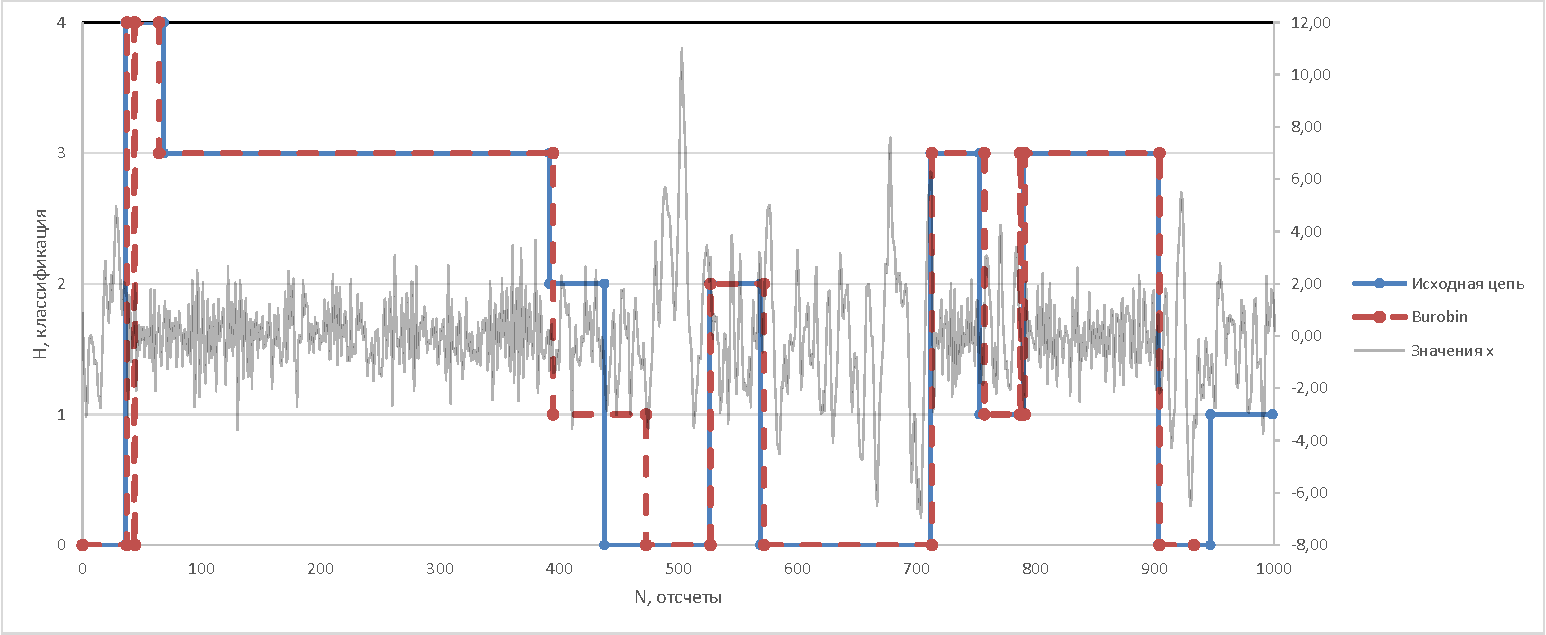
\includegraphics[width=\linewidth]{1k_burobin}
\caption{Сигнал 1, t = 1000}
\end{minipage}
\begin{minipage}[h]{0.49\linewidth}
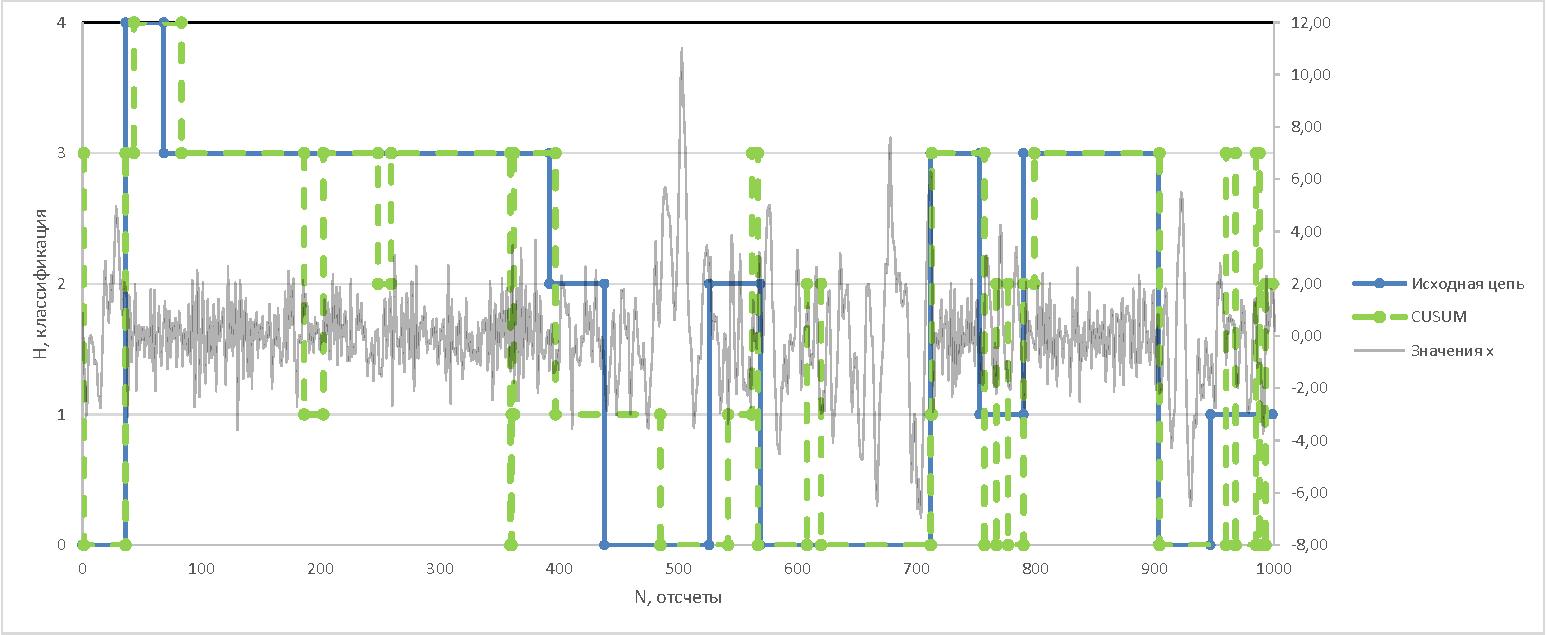
\includegraphics[width=\linewidth]{1k_cusum}
\caption{Сигнал 1, t = 1000}
\end{minipage}
\end{figure}
\end{frame}

\begin{frame}\frametitle{Результаты}
\framesubtitle{Модельный сигнал}
\begin{figure}[h]
\begin{minipage}[h]{0.4\linewidth}
\begin{table}[h]
\caption{Параметры модельного сигнала}
\label{signal_param}
\begin{tabular}{|c|c|c|c|c|}
\hline
h & $\phi_0$ & $\phi_1$ & $\phi_2$ & $B$\\
\hline
0 & 0 & 1.36 & -0.49 & 1\\
\hline
1 & 0 & 1.02 & -0.40 & 1\\
\hline
2 & 0 & 0.82 & -0.49 & 1\\
\hline
3 & 0 & 0 & -0.49 & 1\\
\hline
4 & 0 & -0.82 & -0.49 & 1\\
\hline
\multicolumn{5}{|c|}{$q_{ii} = 0.99$}\\
\hline
\multicolumn{5}{|c|}{$q_{ij} = 0.0025$, $i \neq j$}\\
\hline
\end{tabular}
\end{table}
\end{minipage}
\begin{minipage}[h]{0.4\linewidth}
Было проведено исследование качества обоих алгоритмов. В качестве меры точности алгоритма было взято среднее время совпадения построенной сегментации с оригинальной, усредненное по $N = 20000$ запусков. Были получены следующие результаты:
\end{minipage}
\end{figure}
$$t = 1000,\; Q_B = 0.86795,\; Q_{CUSUM} = 0.76240$$
$$t = 2000,\; Q_B = 0.86408,\; Q_{CUSUM} = 0.75599$$
$$t = 3000,\; Q_B = 0.86235,\; Q_{CUSUM} = 0.75323$$
\end{frame}

\begin{frame}\frametitle{Результаты}
\framesubtitle{Сигнал с вентилятора}
Были произведены 3 записи шума вентилятора в нормальном режиме работы и с разладкой - в работающий вентилятор засовывалась бумажка. Один из сигналов был использован для подбора параметров для алгоритмов. С помощью МНК были определены коэффициенты авторегрессии с глубиной модели $P = 10$. На графиках показаны зависимости коэффициентов авторегрессии для этого сигнала а) до разладки, б) во время разладки от количества отсчетов, анализируемых МНК.
\begin{figure}[h]
\begin{minipage}[h]{0.49\linewidth}
\center{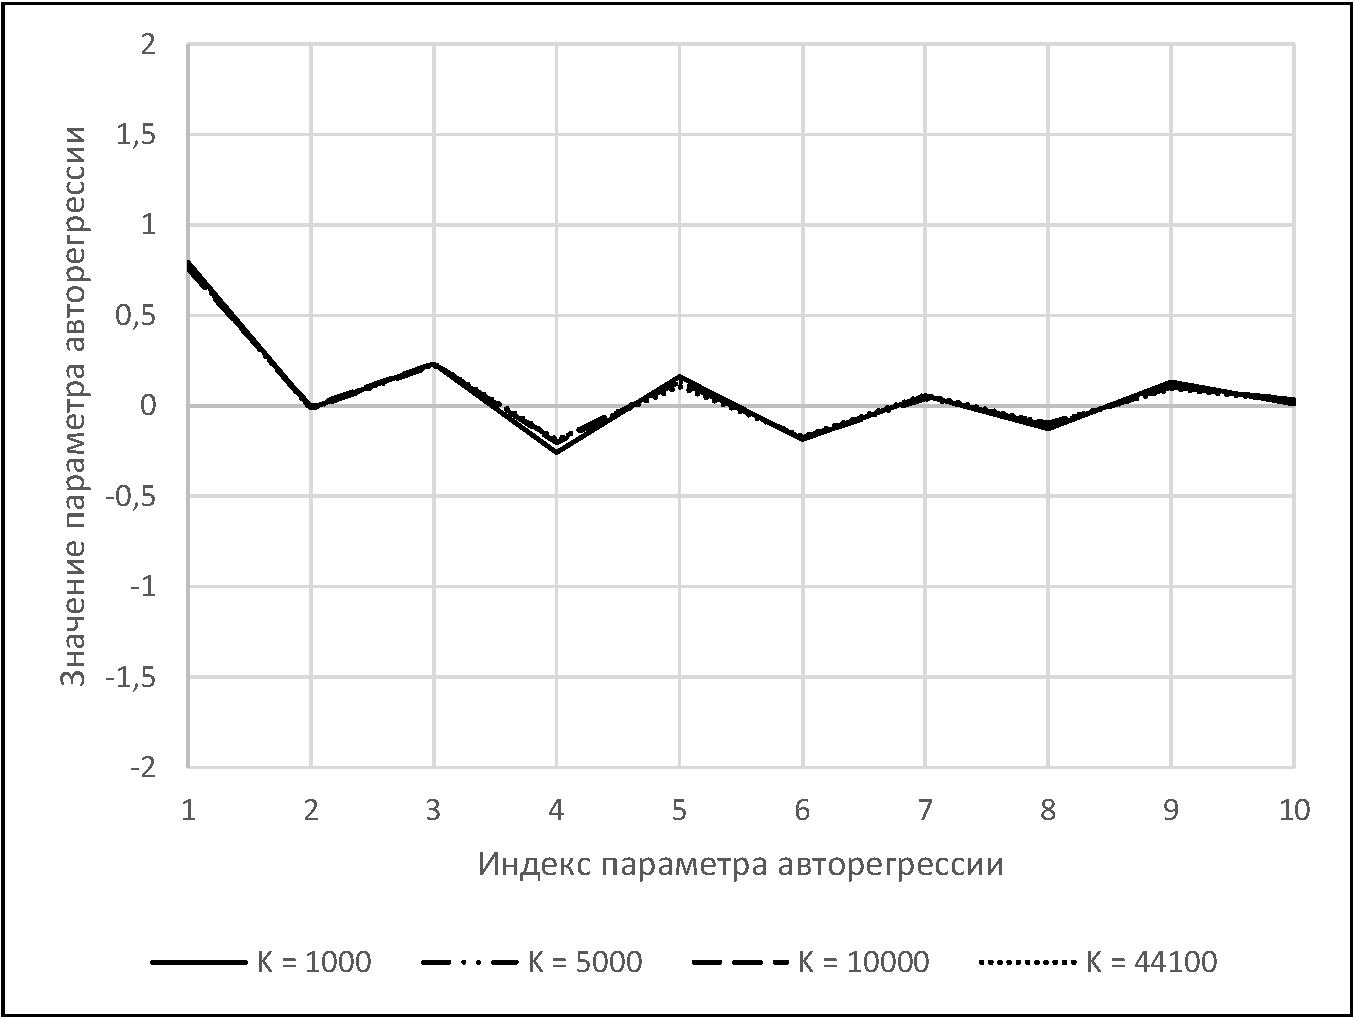
\includegraphics[width=\linewidth]{autoregression_params_normal} \\а)}
\end{minipage}
\begin{minipage}[h]{0.49\linewidth}
\center{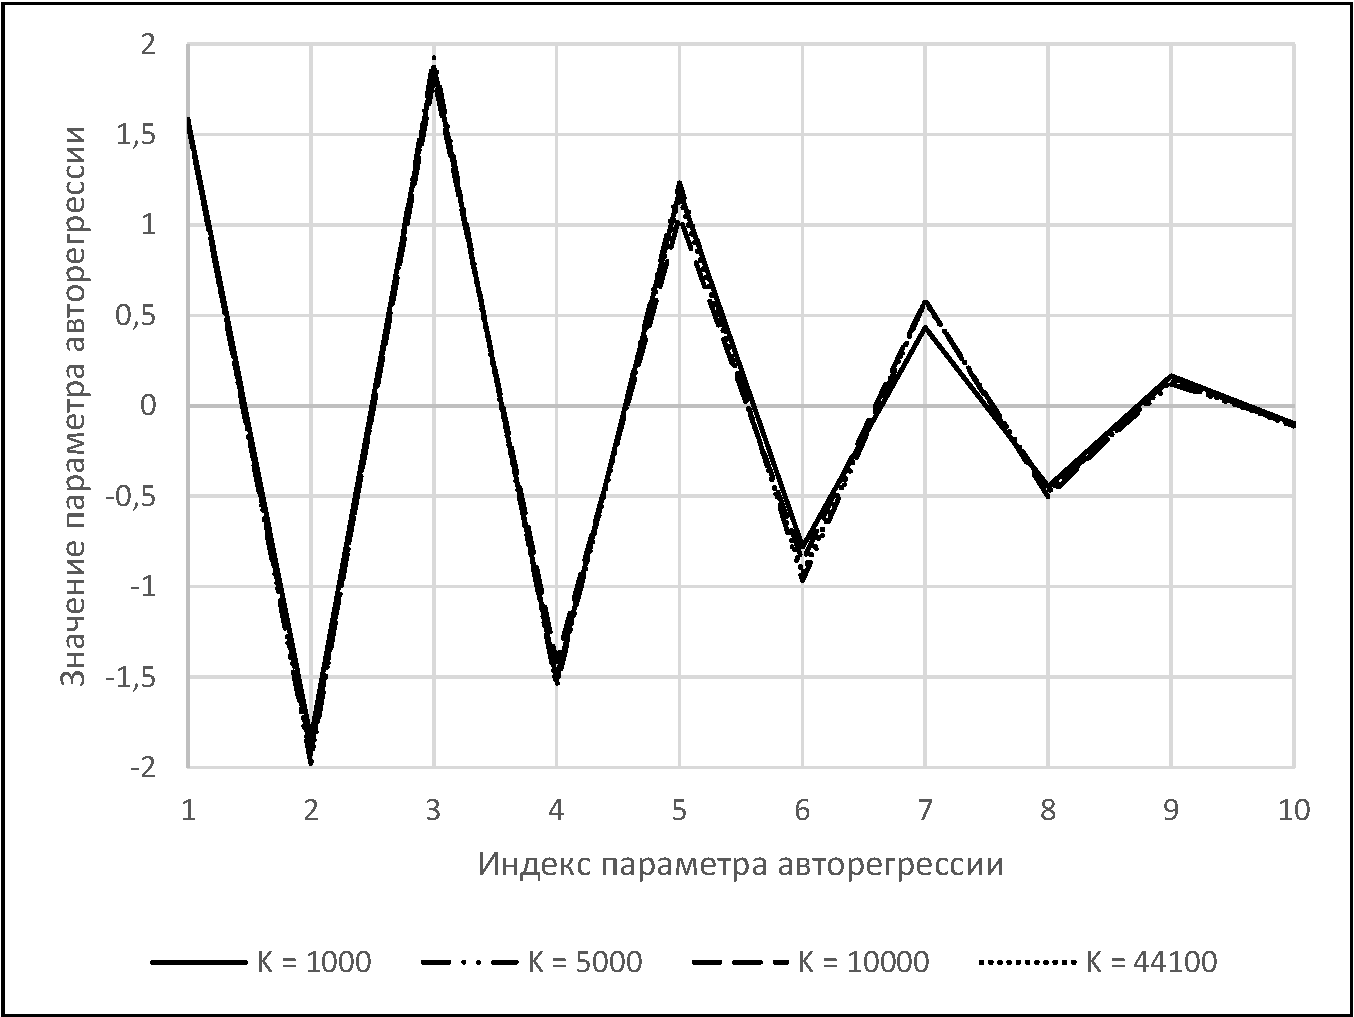
\includegraphics[width=\linewidth]{autoregression_params_disaster} \\ б)}
\end{minipage}
\caption{Значения коэффициентов авторегрессии до и во время разладки}
\end{figure}
\end{frame}

\begin{frame}\frametitle{Результаты}
\framesubtitle{Сигнал с вентилятора}

\begin{table}[h]
\caption{Оценки коэффициентов авторегрессий, полученные МНК}
\begin{tabular}{|c|c|c|c|c|c|c|c|c|c|c|c|c|}
\hline
h & $\phi_0$ & $\phi_1$ & $\phi_2$ & $\phi_3$ & $\phi_4$ & $\phi_5$ & $\phi_6$ & $\phi_7$ & $\phi_8$ & $\phi_9$ & $\phi_{10}$\\
\hline
0 & 0 & 0.78 & 0 & 0.23 & -0.19 & 0.11 & -0.17 & 0.06 & -0.1 & 0.1 & 0\\
\hline
1 & 0 & 1.58 & -1.94 & 1.88 & -1.53 & 1.16 & -0.93 & 0.58 & -0.47 & 0.14 & -0.11\\
\hline
\end{tabular}
\end{table}

В таблице $h_0$ соответствует нормальной работе вентилятора, а $h_1$ - разладке. Подобранные параметры для алгоритмов составили \center{$B(h_i) = 10^5,\; q_{ii} = 0.99999,\; T_{ij} = 4 \cdot 10^6.$}
\begin{figure}[h]
\begin{minipage}[h]{0.49\linewidth}
\center{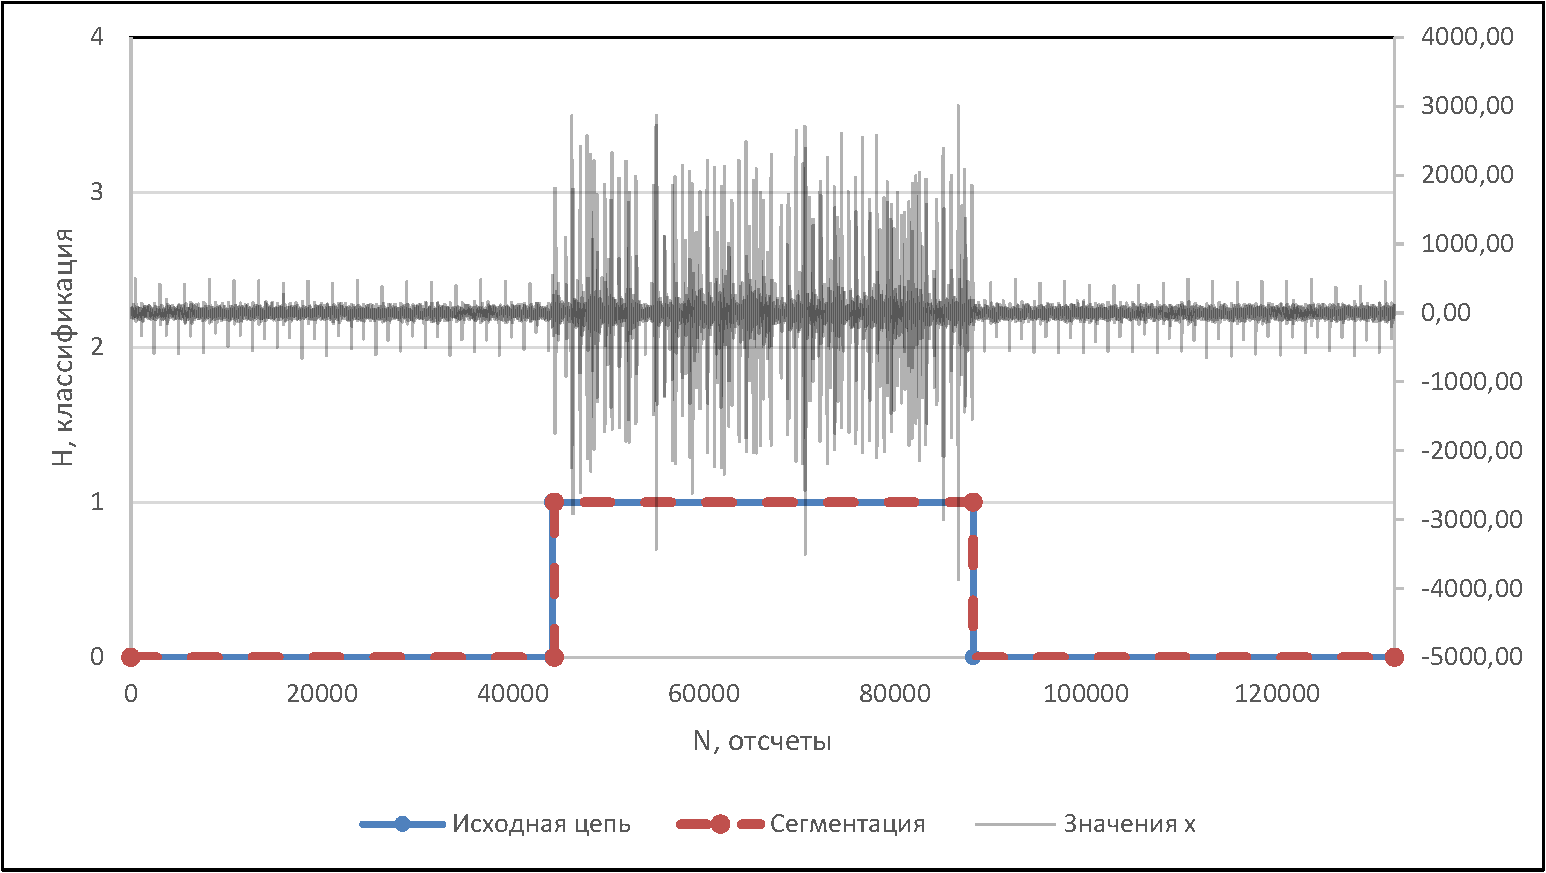
\includegraphics[width=\linewidth]{signal_cropped_1_burobin} \\а)}
\end{minipage}
\begin{minipage}[h]{0.49\linewidth}
\center{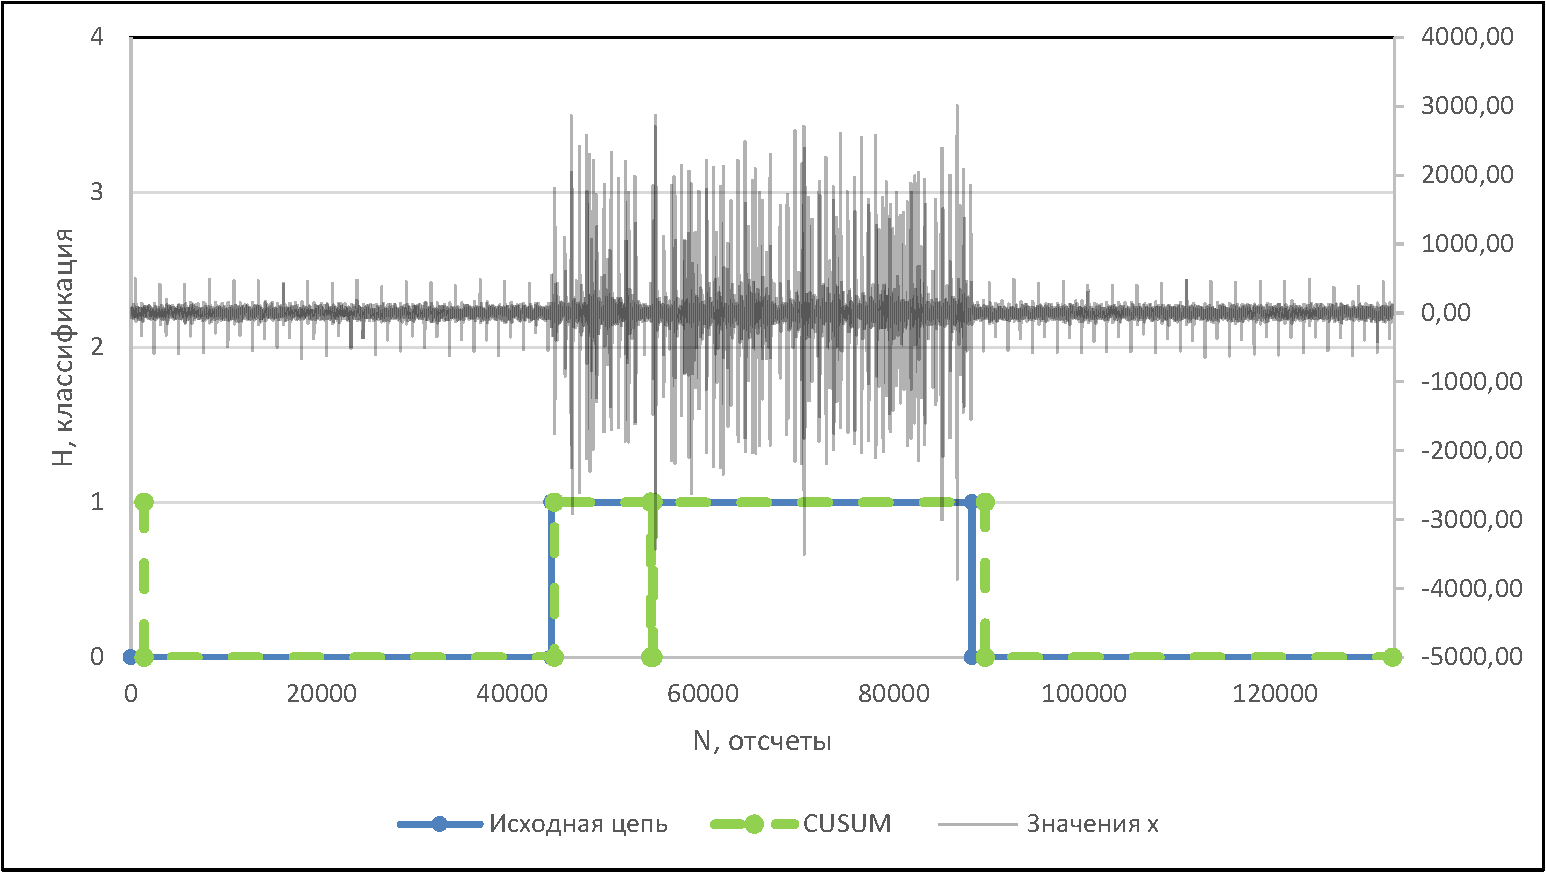
\includegraphics[width=\linewidth]{signal_cropped_1_cusum} \\б)}
\end{minipage}
\caption{Сегментация первого сигнала с вентилятора обоими алгоритмами}
\end{figure}
\end{frame}

\begin{frame}\frametitle{Результаты}
\framesubtitle{Сигнал с вентилятора}
Не изменяя найденных параметров, алгоритмы были применены к другим двум оставшимся сигналам:
\begin{figure}[h]
\begin{minipage}[h]{0.49\linewidth}
\center{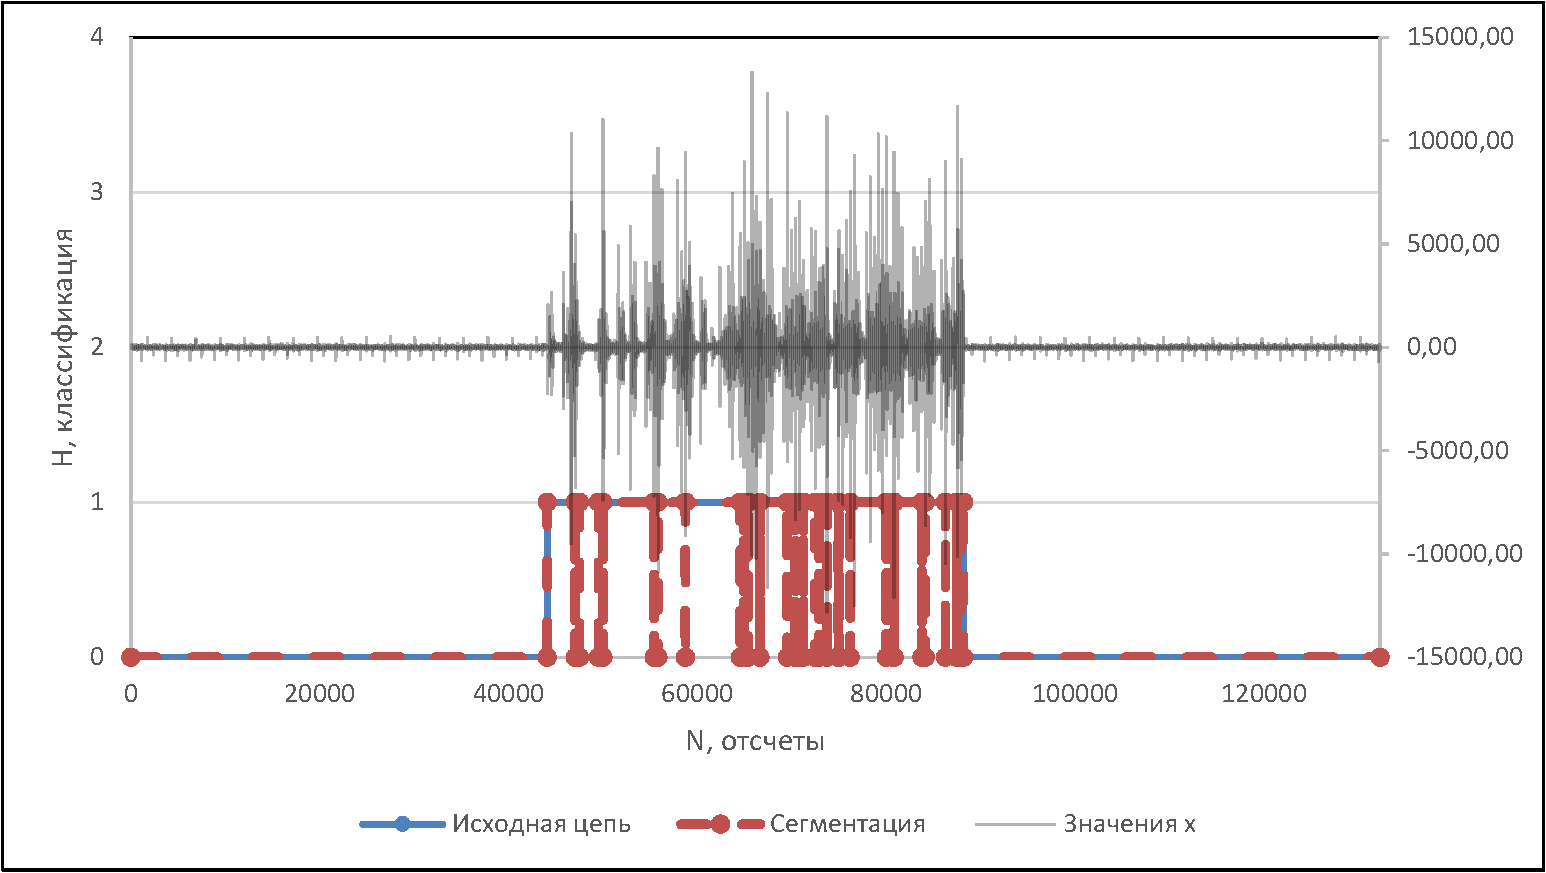
\includegraphics[width=\linewidth]{signal_cropped_2_burobin} \\а)}
\end{minipage}
\begin{minipage}[h]{0.49\linewidth}
\center{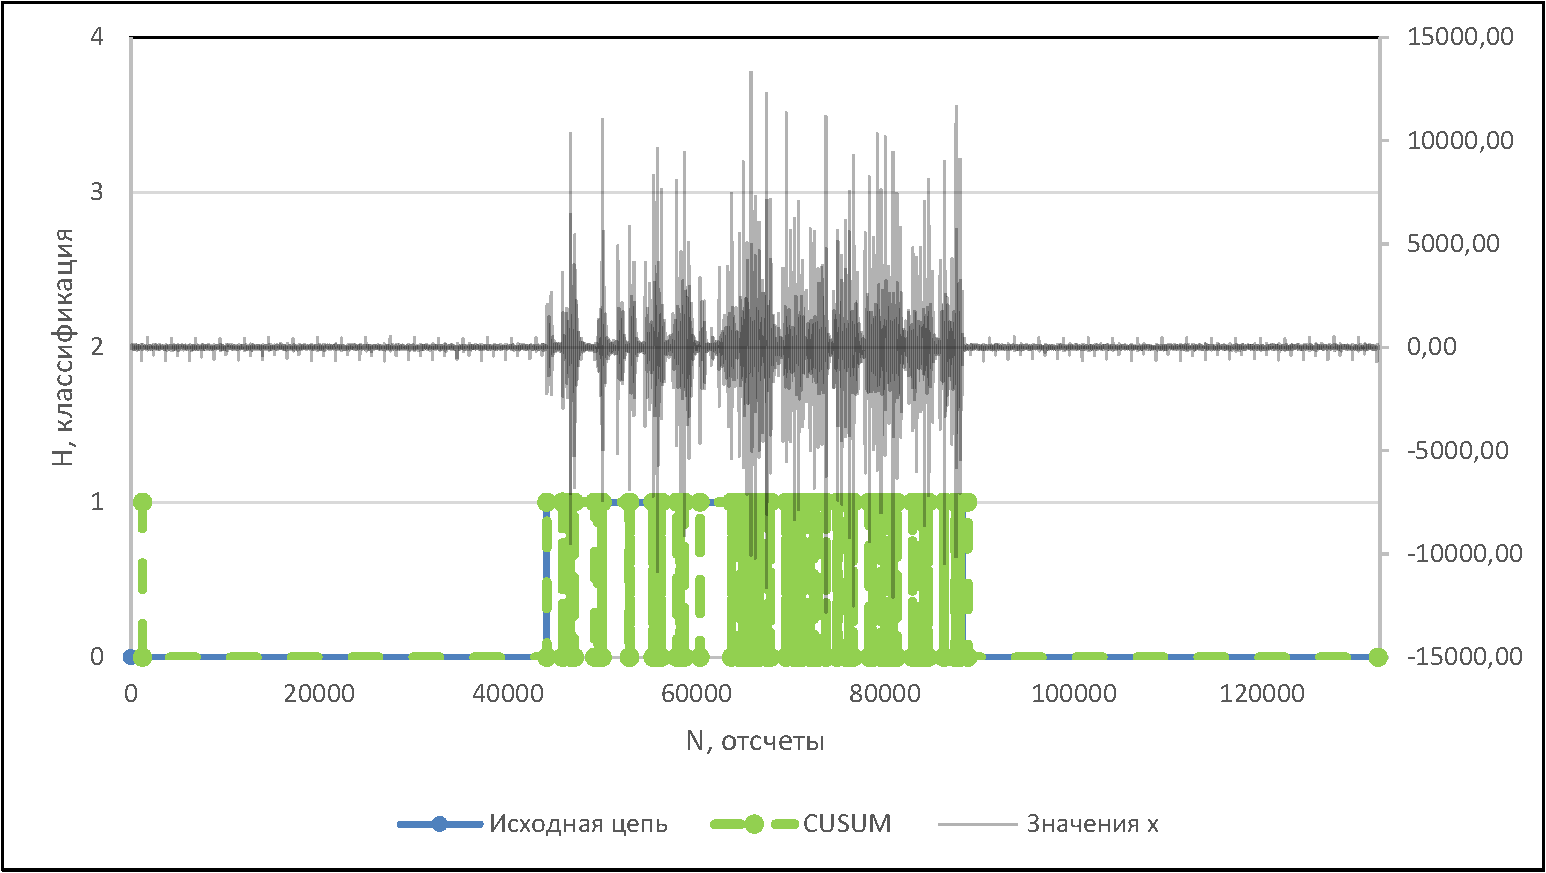
\includegraphics[width=\linewidth]{signal_cropped_2_cusum} \\б)}
\end{minipage}
\caption{Сегментация второго сигнала с вентилятора обоими алгоритмами}
\end{figure}
\end{frame}

\begin{frame}\frametitle{Результаты}
\framesubtitle{Сигнал с вентилятора}

\begin{figure}[h]
\begin{minipage}[h]{0.49\linewidth}
\center{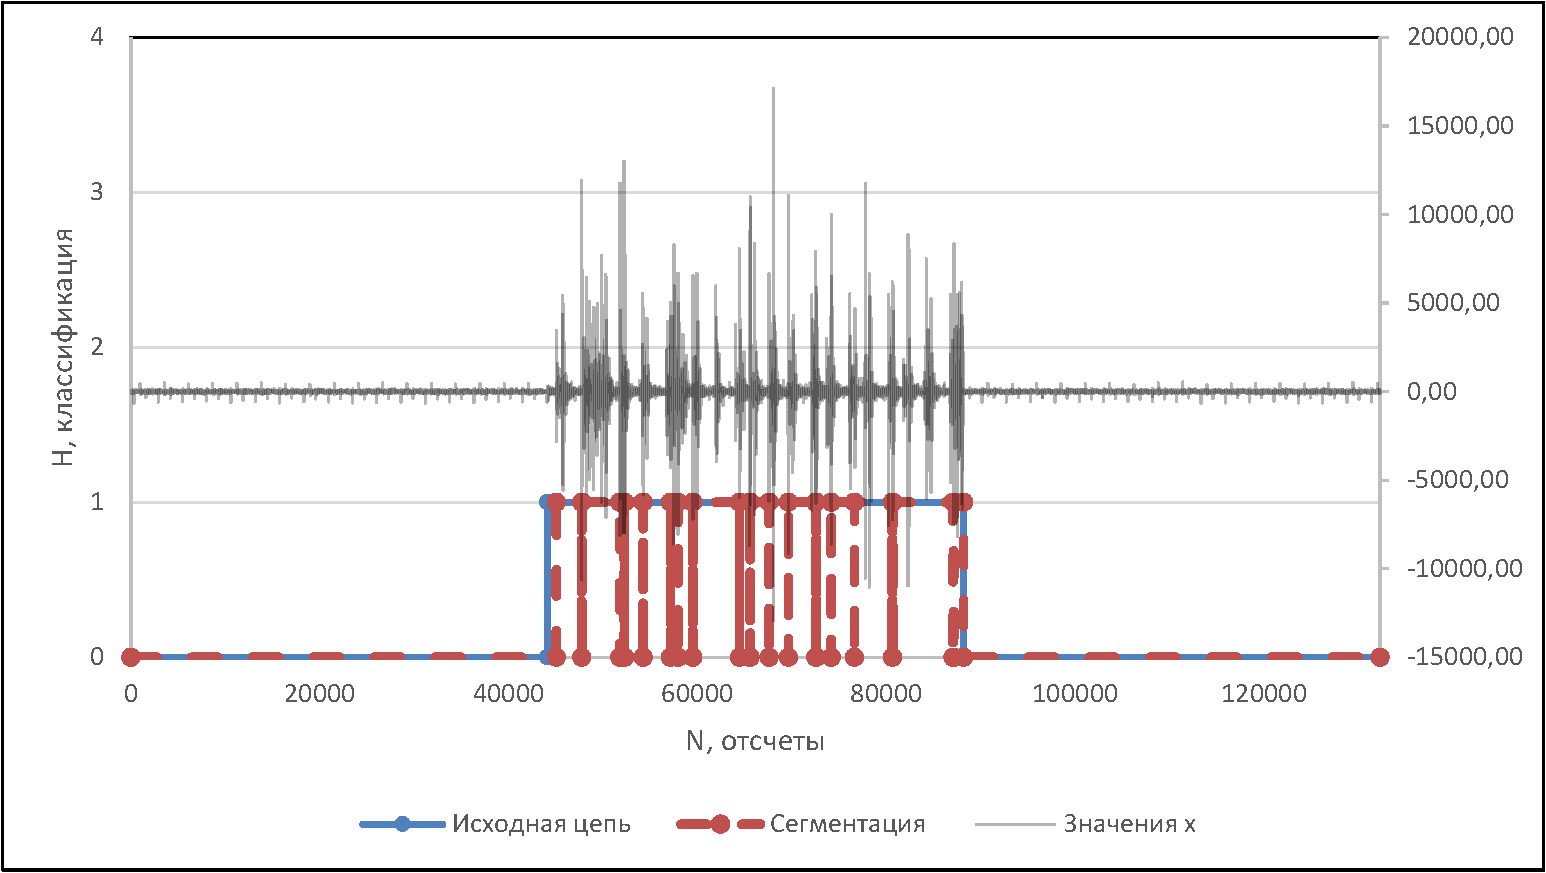
\includegraphics[width=\linewidth]{signal_cropped_3_burobin} \\а)}
\end{minipage}
\begin{minipage}[h]{0.49\linewidth}
\center{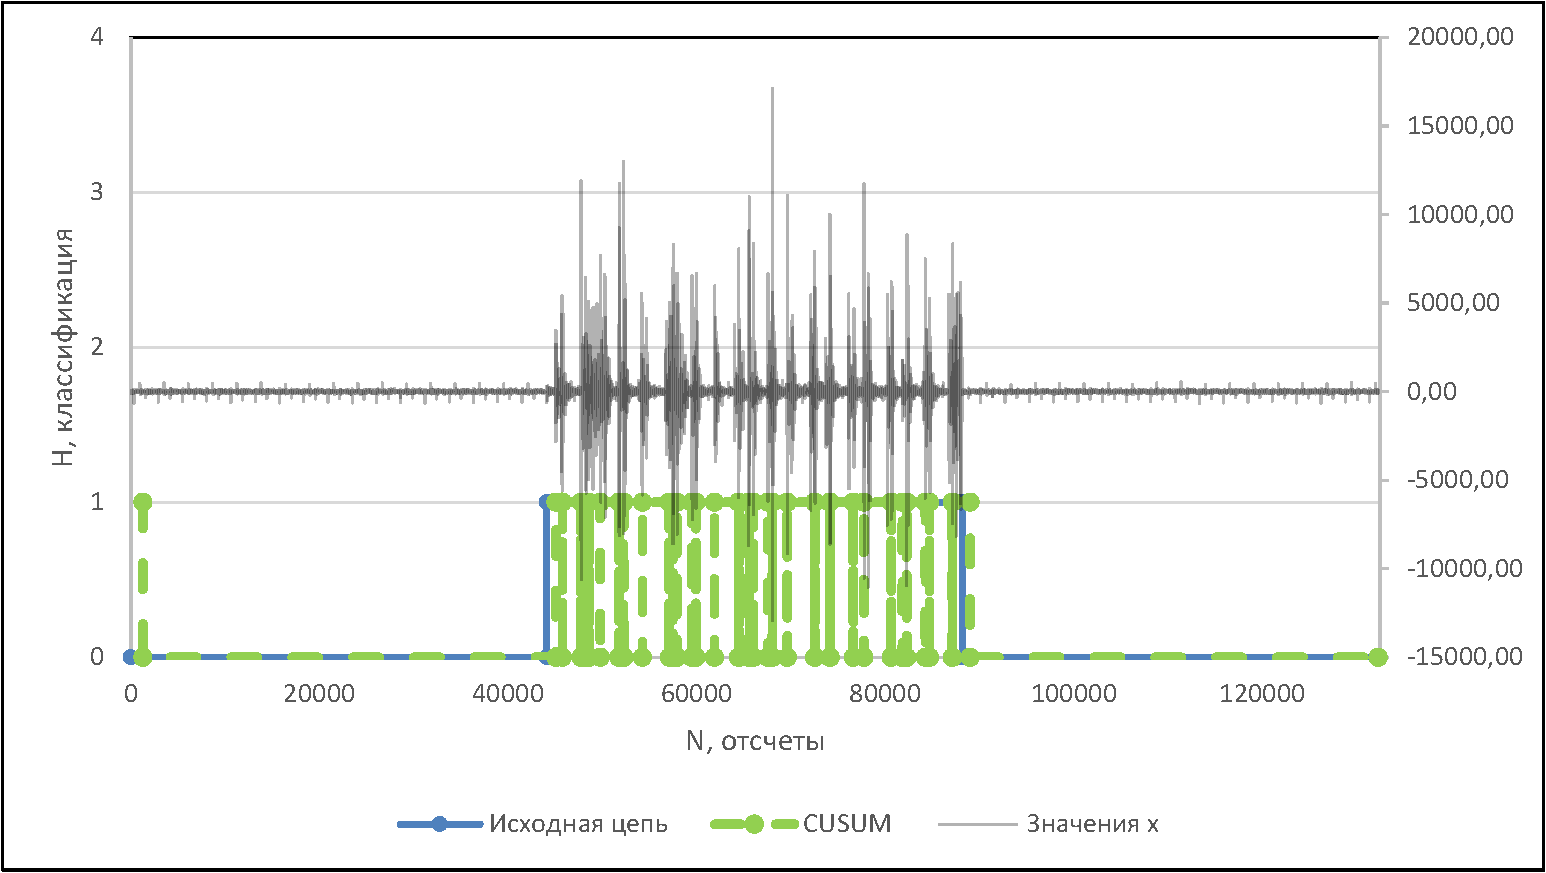
\includegraphics[width=\linewidth]{signal_cropped_3_cusum} \\б)}
\end{minipage}
\caption{Сегментация третьего сигнала с вентилятора обоими алгоритмами}
\end{figure}
\end{frame}

\begin{frame}\frametitle{Выводы}
Результаты, полученные из экспериментов с модельным сигналом показывают, что
\begin{itemize}
\item Aлгоритм на основе метода динамического программирования имеет в среднем на 10 \% большую точность. Это логично, поскольку он учитывает больше данных о входном сигнале, чем CUSUM(а именно вероятности переходов, заданные в матрице $Q$).
\item Алгоритм CUSUM является более легким в реализации и работает быстрее, однако его точность сильно зависит от выбора пороговых значений $T_{ij}$ для каждой пары переходов, что само по себе является довольно неочевидной задачей.
\end{itemize}

Эксперименты на реальном сигнале с электромеханического устройства(вентилятора) показали, что рассматриваемый подход применим к реальным сигналам, однако требует некоторой доработки.
\end{frame}
\end{document}